\section{Computational Experiment}
In this section, we select Continuous MountainCar, SparseHalfCheetah and HalfCheetah three tasks as benchmarks to evaluate the method we proposed, representing deceptive rewards, sparse rewards, and well-defined tasks. We use the vanilla Deep Deterministic Policy Gradient algorithm as the no exploration baseline and implement the action noise, parameter noise version as a comparison to our method. By visualizing the variance of the critic in the state-action space, we demonstrate that SGLD-based exploration strategy generates intrinsic motivation in sparse environments. The evaluation results of the four methods on the three benchmarks are given and compared. We used uniform settings on all three tasks and solved all the tasks, surpassing other methods.

\subsection{Experiment Setting}
For each task, we run the training process six times with different random seeds (which are the same for different exploration strategies). For each training process, we train the agent with $1\times10^6$ transition data and evaluate the agent with the learning policy(different from the rollout policy) for ten times to get the average value of non-discount total return. More experiment setting is available in Appendix \ref{apdx:detail}.

\subsubsection{CMC, HC, and SHC}
We selected three continuous state-action space control tasks with different reward attributes as benchmarks, and all environments were modified from the original gym environments \cite{gym}.

\textbf{Continuous MountainCar (CMC)}\cite{MC}: In the CMC, the agent needs to control a car from the bottom of the valley to the goal on the mountain top. The agent obtained reward $r = -\alpha*||\vec{a_t}||^2_2 + r_{goal}$ in each time step and the goal reward $r_{goal}=100$ only if the car reach the goal or zero otherwise. The car needs to climb the left side first and then rush to the right side to reach the top of the mountain, otherwise it can only oscillate back and forth in the valley. The Continuous MountainCar is a task with both sparse rewards and action penalties.

\textbf{HalfCheetah (HC)}: As described in Section \ref{sec:tasks}, the agent needs to control a half cheetah to run as fast as possible to the right with minimal control. The HalfCheetah is a well-defined task with the default $\alpha = 0.1$, but as $\alpha$ increases, exploration becomes more and more difficult.

\textbf{Sparse HalfCheetah (SHC)}: The SHC removes the action penalty from the HC and only receives a reward of 1 for each time step after the cheetah moves to the right beyond the distance $d$. Obviously, as distance $d$ increases, it is more difficult for any random strategy to get a non-zero reward.

\begin{figure}[htb]
   \centering  
   \subfigure[Continuous MountainCar]{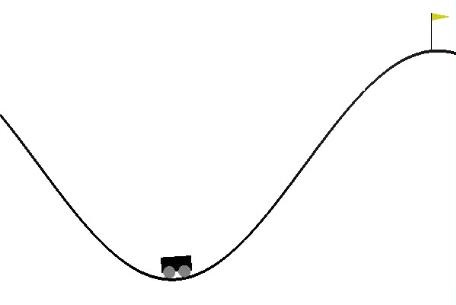
\includegraphics[width=100pt]{figs/MC.jpg}}
   \subfigure[HalfCheetah]{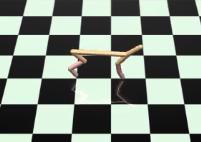
\includegraphics[width=100pt]{figs/HC.jpg}}
   \caption{Snapshot of the gym environment.}
   \label{fig:MC}
\end{figure}

\subsubsection{Deep Deterministic Policy Gradient}
\textbf{Deep Deterministic Policy Gradient (DDPG)} is an off-policy actor-critic algorithm that uses a replay buffer and two target networks \cite{DDPG}. In each training cycle, the agent rollouts some transition data from the environment $E$ and stores them into the replay buffer $D$. Then the algorithm calculate the Bellman Error by Equation (\ref{eq:bellman}) with the target network $Q'$ and $\mu'$ and optimize the parameters $\theta^{Q}$ of the critic $Q$ in several training steps, and optimize the parameters $\theta^{\mu}$ of the actor $\mu$ by the policy gradient estimated by the critic. The target network is soft updated at the end of each training step. The details of the algorithm are described in Algorithm \ref{alg:DDPG}.
\begin{equation}
   \label{eq:bellman} 
   \begin{aligned}
   L^Q=\mathbb{E}_{s_t\sim\rho^{\tilde\mu},a_t\sim\tilde\mu,r_t\sim E}[(Q(s_t,a_t)-y_t)^2]\\
   \text{where\quad}  y_t = \gamma Q'(s_{t+1},\mu'(s_{t+1}))+r_t
   \end{aligned}
\end{equation}

Since DDPG is an off-policy algorithm, the rollout actor and the learning actor do not need to be the same, the exploration strategy $f(\cdot) : \mathbb{M} \rightarrow \mathbb{M}$, where $\mathbb{M}$ is the space of policy, commonly transforms the learning actor $\mu$ into a rollout actor $\tilde\mu$ to achieve exploration.

\begin{algorithm}[htbp]
   \caption{Deep Deterministic Policy Gradient}
   \label{alg:DDPG}
\begin{algorithmic}
   \STATE {\bfseries Input:} environment $E$, critic $Q(s,a|\theta^Q)$, actor $\mu(s|\theta^\mu)$, exploration strategy $\tilde\mu \leftarrow f(\mu)$
   \STATE Initialize replay buffer $D = \emptyset$.
   \STATE Initialize target network $Q'= Q$, $\mu'= \mu$.
   \FOR{1 {\bfseries to} cycle\_number}
   \STATE Apply exploration strategy $\tilde\mu \leftarrow f(\mu)$
   \STATE Rollout data $d_t$ from $E$ by $\tilde\mu$ and $D \leftarrow D\cup {d_t}$

   \FOR{1 {\bfseries to} train\_steps}
   \STATE Sample data batch $\{d_t=(s_t,a_t,r_t)\}$ from $D$
   \STATE $L^Q=\sum(\gamma Q'(s_{t+1},\mu'(s_{t+1}))+r_t-Q(s_t,a_t))^2$
   \STATE $L^\mu=-\sum Q(\mu(s_t))$
   \STATE $\theta^Q \leftarrow \theta^Q - \alpha^Q\cdot\nabla_{\theta^Q} L^Q$
   \STATE $\theta^\mu \leftarrow \theta^\mu -\alpha^\mu\cdot\nabla_{\theta^\mu} L^\mu$
   \STATE Soft update target network $Q'$ and $\mu'$
   \ENDFOR
   \ENDFOR
\end{algorithmic}
\end{algorithm}

In original DDPG algorithm, the target networks are the $\tau$-moving average of parameters of actor and critic. After each gradient descent step on actor and critic ,the target networks are "soft updated" by Equation (\ref{eq:soft}).
\begin{equation}
\label{eq:soft} 
\begin{aligned}
\theta^{Q'} = (1-\tau)\theta^{Q'}+\tau\theta^Q\\
\theta^{\mu'} = (1-\tau)\theta^{\mu'}+\tau\theta^\mu
\end{aligned}
\end{equation}

The optimized object for the critic in one cycle is minimizing Bellman error in Equation (\ref{eq:bellman}), which is associated with both data in replay buffer and the target network. Constantly updating the target during the training step will make the process of sampling from the posterior distribution inconsistently. In order to sample critic from posterior distribution more strictly, we remain the target unchanged in one cycle and do "hard update", directly copy parameters of actor and critic to target networks. Under this setting, the expectation policy gradient will be integrated over both $s_t\sim\rho$ and $\theta^Q\sim p(\theta^Q|D)$ as Equation (\ref{eq:pg}). 
\begin{equation}
   \label{eq:pg} 
   \begin{aligned}
   \nabla_{\theta^\mu}\mathbb{E}[L^\mu|D] = \mathbb{E}_{s_t\sim\rho,\theta^Q\sim p(\theta^Q|D)}[\nabla_{\theta^\mu}L^\mu]\\
   \end{aligned}
\end{equation}
It is proven to be the correct form to estimate policy gradient with critics sampled from posterior distribution \cite{dropoutInference}.

\subsection{Intrinsic Motivation in State-Action Space}
In the CMC task, the state space is a two-dimensional space composed of position and velocity. To show how SGLD is intrinsically motivated, we visualize the uncertainty of $Q(s,a)$. The agent fixes a=1 and rollout the data, the car will reciprocate, and the observed data is a circle in the phase space. We then use this data to train the Adam version and the SGLD version of the DDPG, and record 50 critic samples, collect the surfaces of these samples on the State plane, and calculate the variance at each point, as shown in Figure \ref{fig:stateaction}.

\begin{figure}[htb]
   \begin{center}   
   \centerline{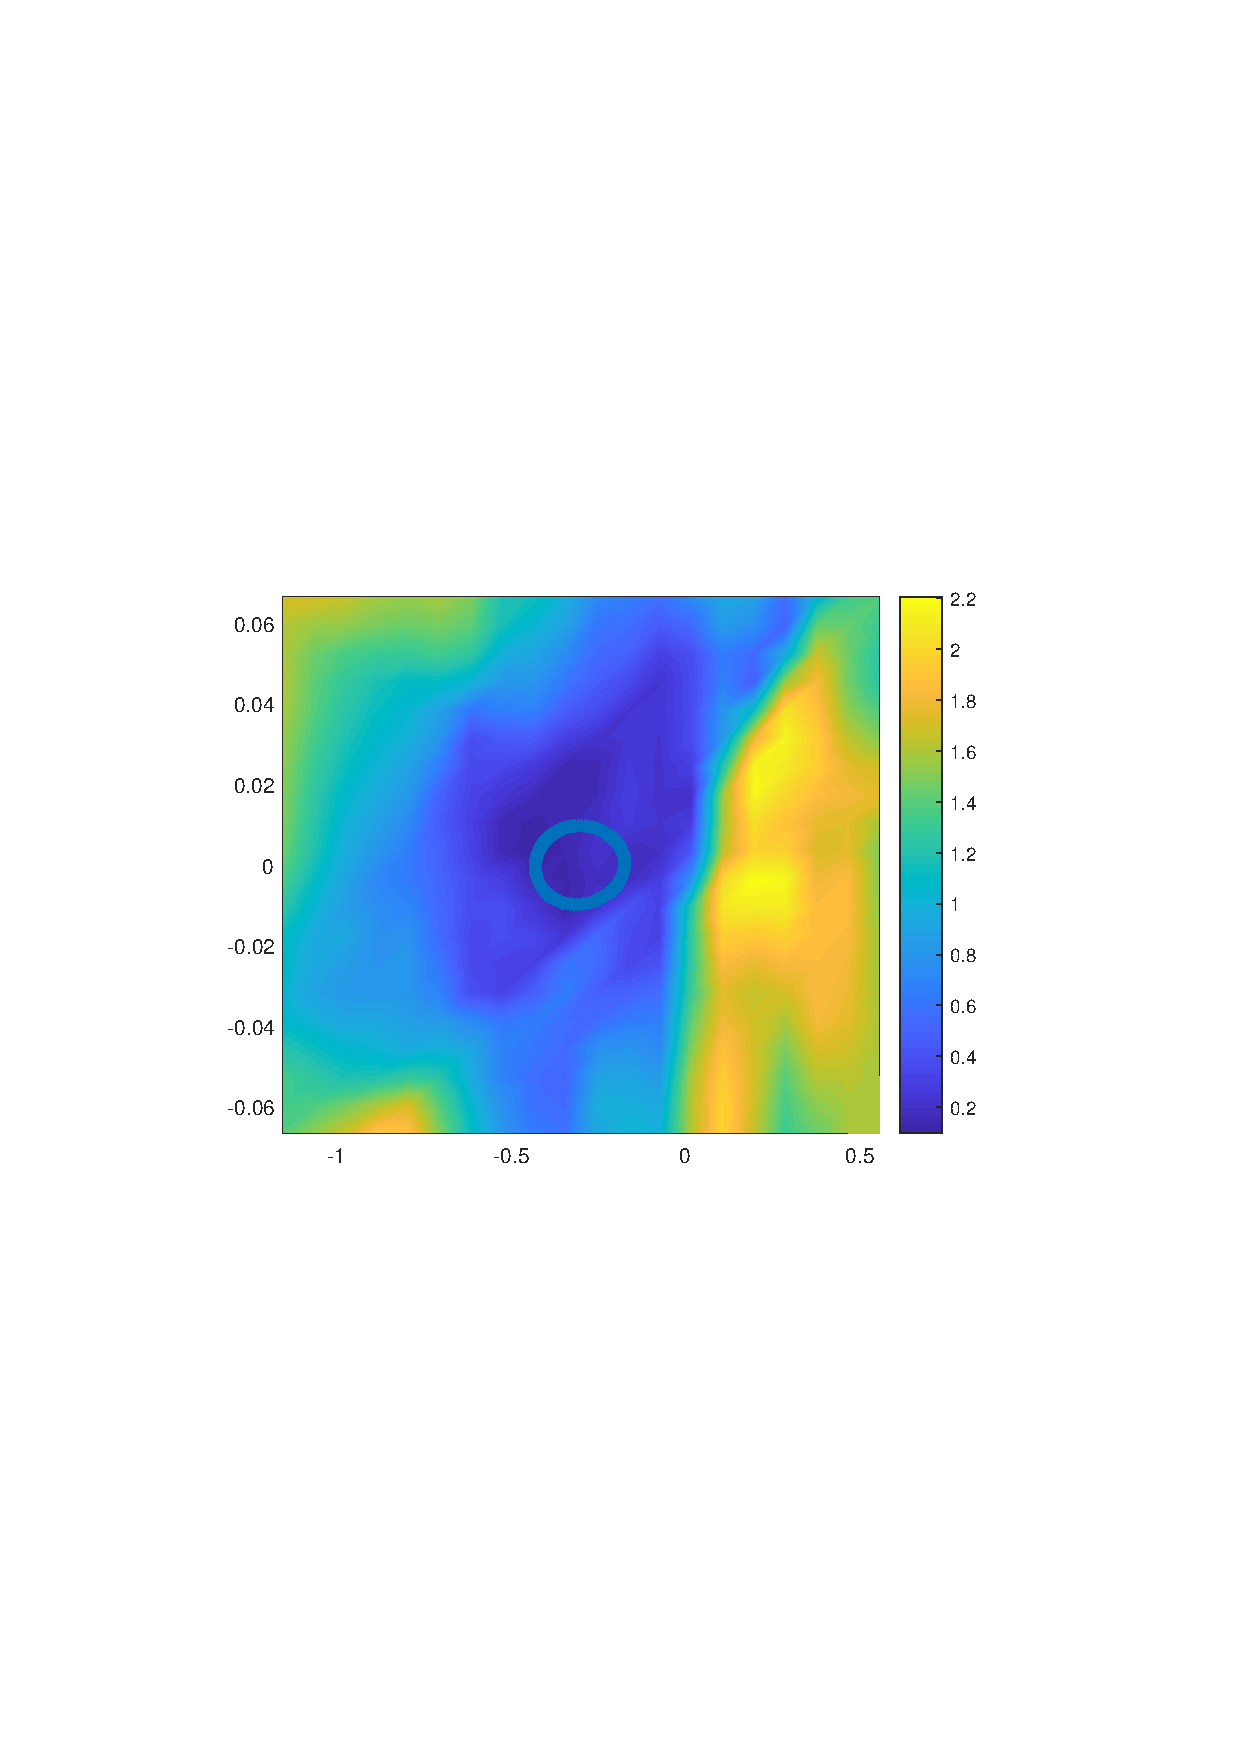
\includegraphics[width=190pt,trim=100 280 100 280,clip]{figs/mc_sgld_state.pdf}}
   \caption{The variance plot of critics sampled by SGLD on Continuous MountainCar}
   \label{fig:stateaction}   
   \end{center}
\end{figure}
As can be seen from the figure: In Adam version, the critic converges to a unique output of zero and the variance is almost 0 over the entire plane. In SGLD version, the critic has a smaller variance near the data circle, and a larger variance in the far away area. The results show that SGLD can correctly describe the posterior distribution of critic.

\subsection{Exploration and Exploitation}
We evaluate the performance of our method on CMC, HC, and SHC and compare it with the results of no exploration baseline, action noise, and parameter noise.

On the CMC, including no action penalty, no exploration and parameter noise all failed. The action noise and SGLD methods succeed with high probability under all conditions. As the action penalty increases, the probability of the SGLD solving the task decreases, but the action noise is almost unaffected. This phenomenon is because the Ornstein-Uhlenbeck process can almost always ignore the subject strategy to achieve the goal in the case of std=0.6, which leads to reaching the goral unconditionally, but this success is difficult to extend to other tasks.

\begin{table}[htbp]
   \caption{Number of Succeeded Seed on Continuous MountainCar}
   \label{tab:mc}
   \vskip 0.15in
   \begin{center}
   \begin{tabular}{lcccc}
   \toprule
   $\alpha$ & Baseline & SGLD & AN & PN \\
   \midrule
      0     & 0        & 6    & 6  & 0 \\
      0.1   & 0        & 6    & 5  & 0 \\
      0.2   & 0        & 5    & 6  & 0 \\
      0.5   & 0        & 4    & 6  & 0 \\
      0.1   & 0        & 3    & 6  & 0 \\
   \bottomrule
   \end{tabular}
   \end{center}
   \vskip -0.1in
   \end{table}

On the HC, as the action penalty increases, the task becomes difficult to explore. Under the settings of $\alpha=0$, 0.1 and 0.2, all algorithms showed a consistent learning curve despite different learning speeds. The results suggest that all exploration strategies work under these conditions. When $alpha=0.5$ and 1, the no exploration and action noise methods almost fail, and the parameter noise SGLD method can still maintain the same learning curve as before. We think this is because the rollout policy of the two exploration methods gives the same action in the same state, and the action noise cannot give a consistent action, and the no exploration is difficult to explore due to the action penalty.

\begin{table}[htbp]
   \caption{Average Return on HalfCheetah}
   \label{tab:HC}
   \vskip 0.15in
   \begin{center}
   \begin{tabular}{lcccc}
   \toprule
   $\alpha$ & Baseline & SGLD & AN   & PN \\
   \midrule
   0        & 3843     & 3742 & 3454 & 3776 \\
   0.1      & 2813     & 4091 & 1683 & 2977 \\
   0.2      & 2352     & 3678 & 931  & 2801 \\
   0.5      & 214      & 2464 & 3    & 1641 \\
   1        & 481      &  984 & 684  & 1605 \\
   \bottomrule
   \end{tabular}
   \end{center}
   \vskip -0.1in
   \end{table}
%      0     & $3843\pm1669$& $3742\pm901$& $3454\pm645$& $3776\pm1340$ \\
%0.1   & $2813 \pm 1495$   & $4091 \pm 831$ & $1683\pm823$  & $2977\pm1714$ \\
%0.2 & $2352\pm1399$ & $3678\pm689$ & $931\pm798$ & $2801\pm2298$\\
%0.5 & $214\pm650$ & $2464\pm1883$ & $3\pm19$ & $1641\pm2596$ \\


On the SHC, at the distance $d=1$, the three exploration strategies successfully solved the problem, even the no exploration baseline has one seed reached non-zero rewards. As the interval $d$ increases, the probability that baseline and action noise can explore non-zero rewards is getting lower and lower. However SGLD and parameter noise are stable to solve the problem, which further confirms the conclusion about deep exploration that we obtained on HC.

\begin{table}[htbp]
   \caption{Number of Succeeded Seed on Sparse HalfCheetah}
   \label{tab:shc}
   \vskip 0.15in
   \begin{center}
   \begin{tabular}{lcccc}
   \toprule
       d    & Baseline & SGLD & AN & PN \\
   \midrule
      1     & 1        & 6    & 6  & 6 \\
      2.5   & 0        & 5    & 1  & 6 \\
      5     & 0        & 6    & 0  & 5 \\
      10    & 0        & 4    & 0  & 5 \\
      20    & 0        & 4    & 0  & 2 \\
   \bottomrule
   \end{tabular}
   \end{center}
   \vskip -0.1in
\end{table}

\begin{figure*}[htb]
   \centering
      \subfigure[MC : $\alpha = 0$]{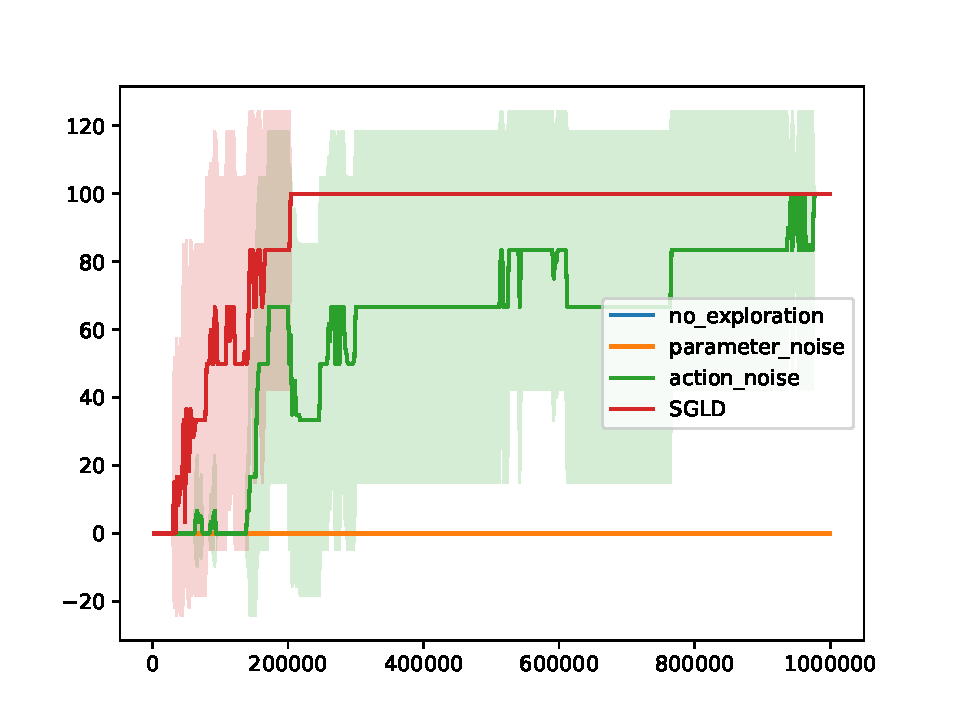
\includegraphics[width=85pt]{figs/MC0.pdf}}
      \subfigure[MC : $\alpha = 0.1$]{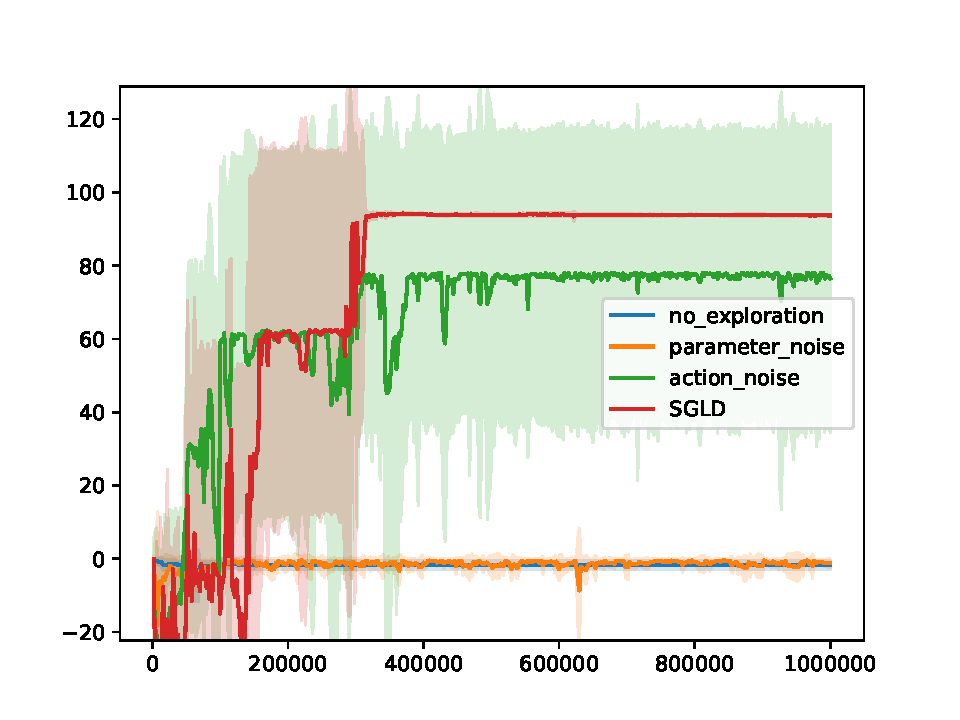
\includegraphics[width=85pt]{figs/MC.pdf}}
      \subfigure[MC : $\alpha = 0.2$]{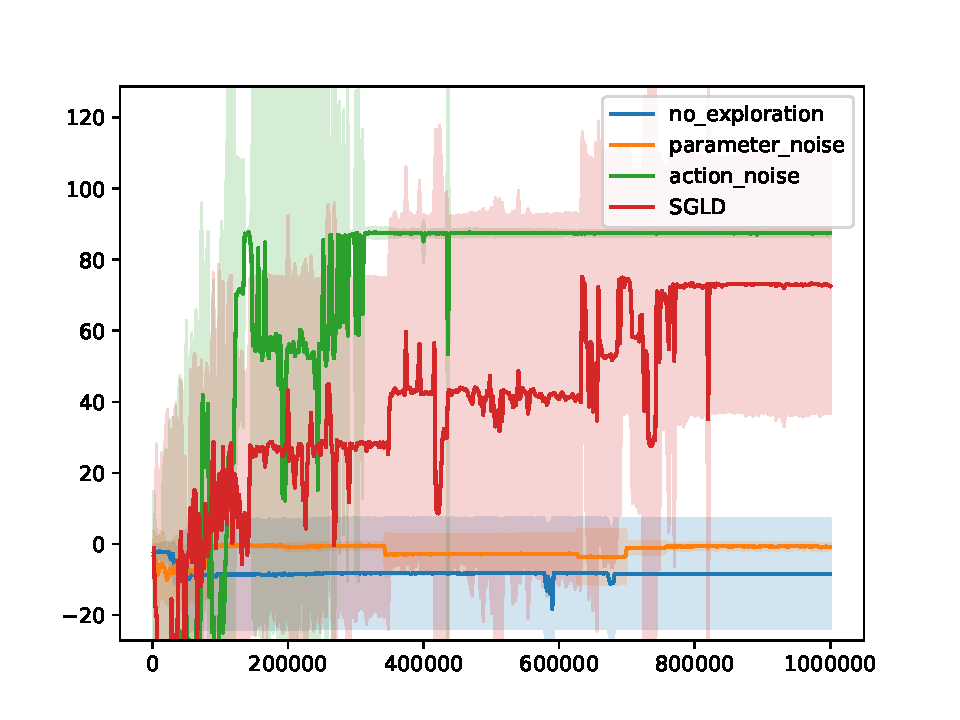
\includegraphics[width=85pt]{figs/MC0_2.pdf}}
      \subfigure[MC : $\alpha = 0.5$]{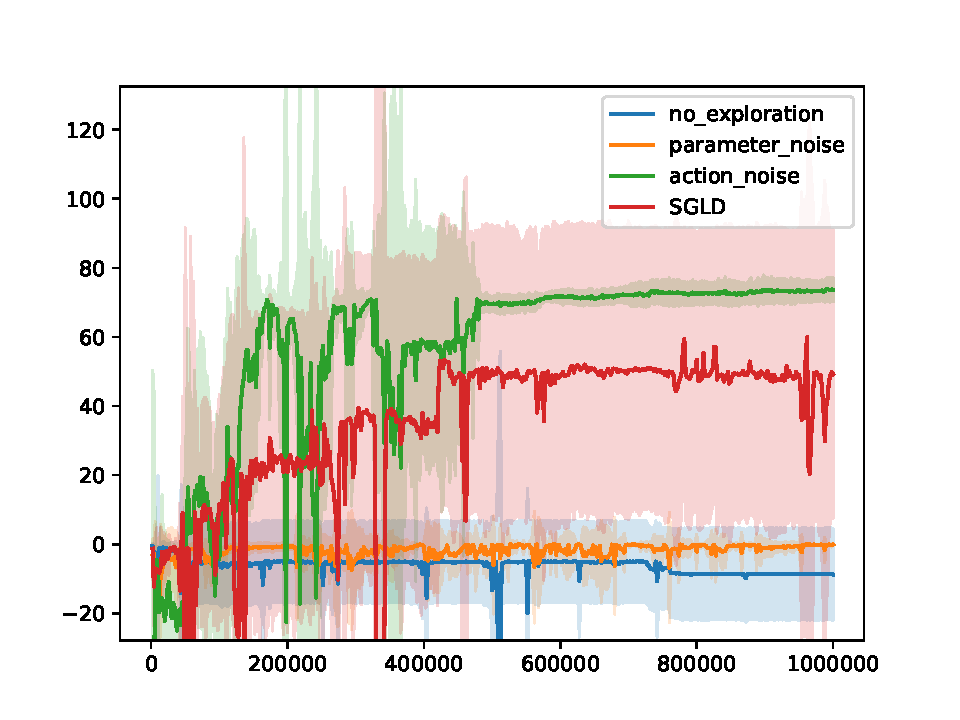
\includegraphics[width=85pt]{figs/MC0_5.pdf}}
      \subfigure[MC : $\alpha = 1$]{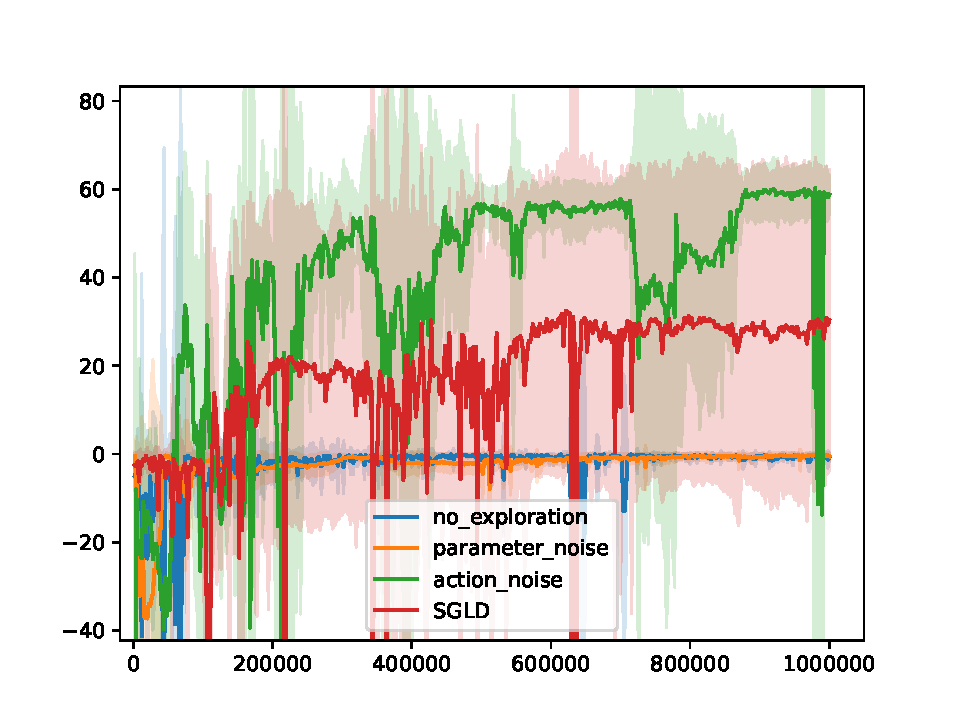
\includegraphics[width=85pt]{figs/MC1.pdf}}
      \subfigure[HC : $\alpha = 0$]{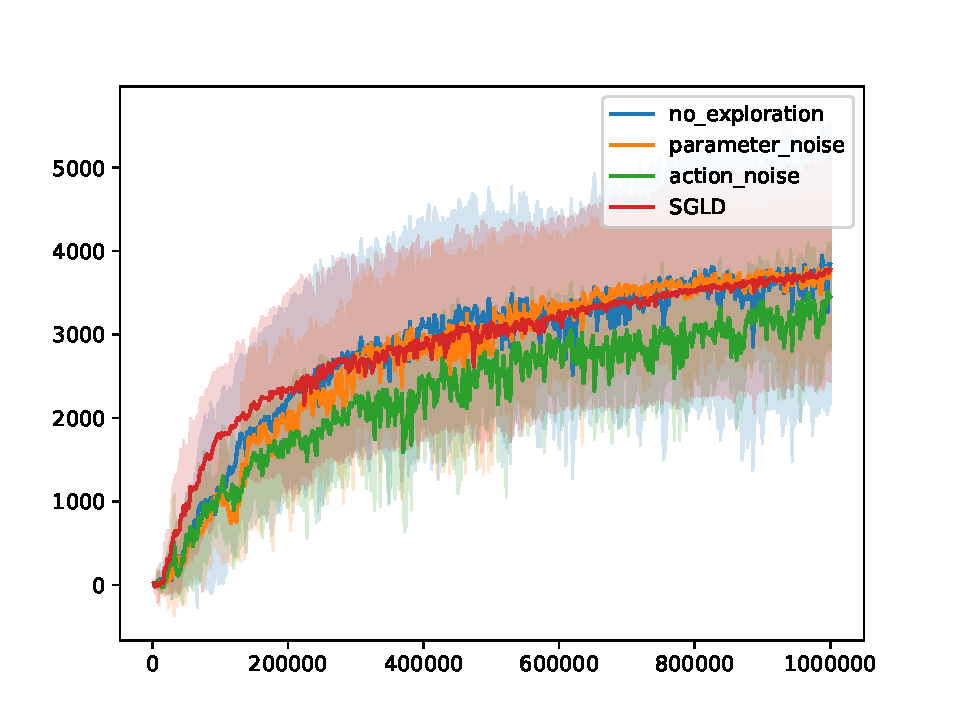
\includegraphics[width=85pt]{figs/HC0.pdf}}
      \subfigure[HC : $\alpha = 0.1$]{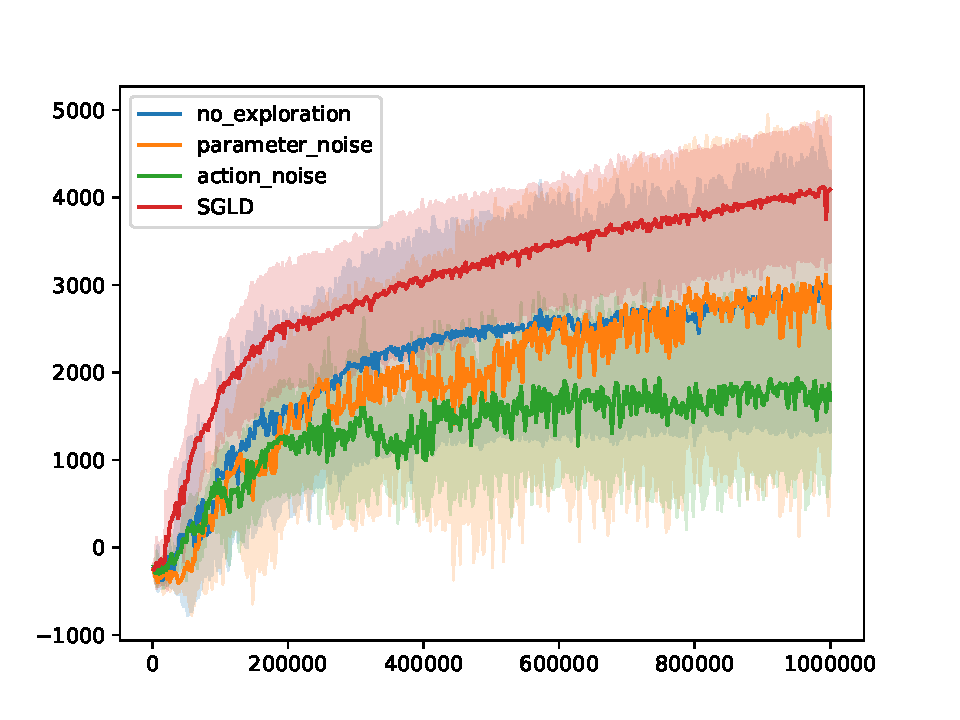
\includegraphics[width=85pt]{figs/HC.pdf}}
      \subfigure[HC : $\alpha = 0.2$]{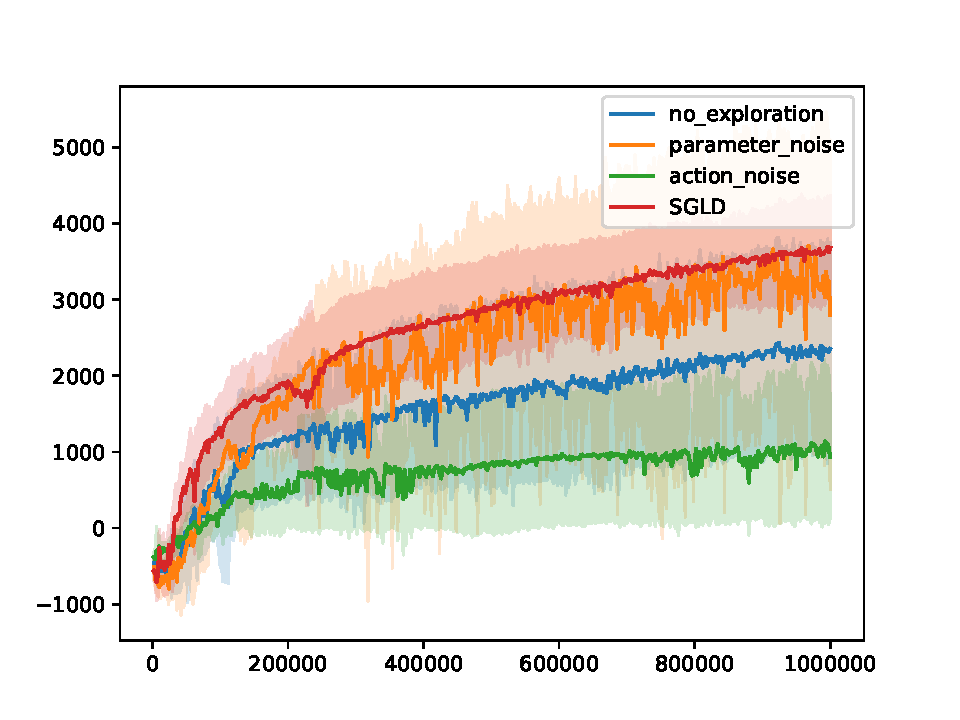
\includegraphics[width=85pt]{figs/HC0_2.pdf}}
      \subfigure[HC : $\alpha = 0.5$]{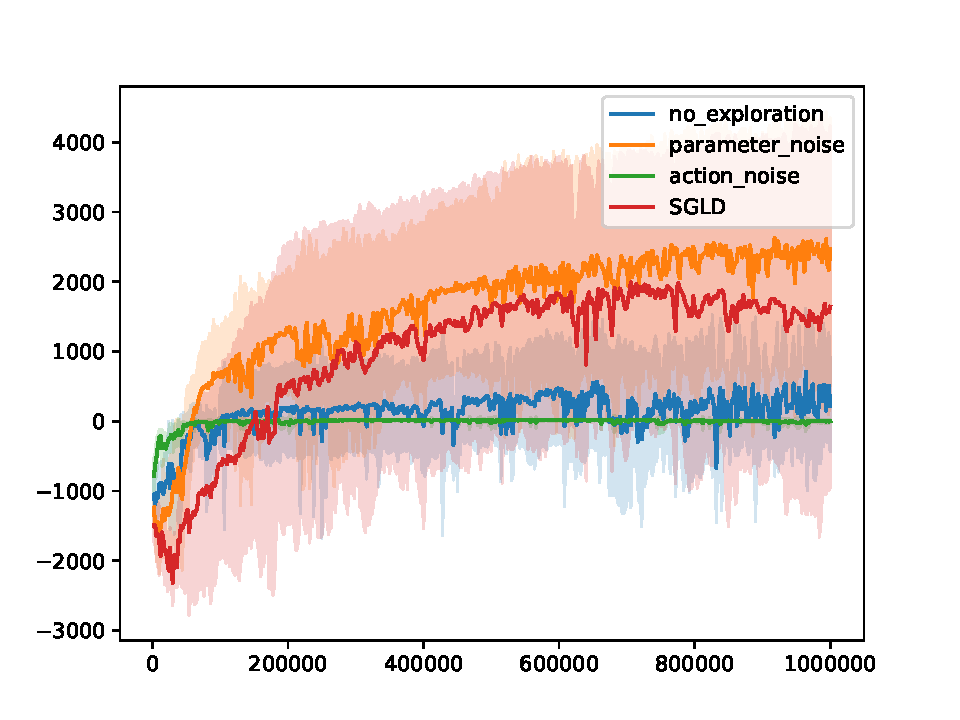
\includegraphics[width=85pt]{figs/HC0_5.pdf}}
      \subfigure[HC : $\alpha = 1$]{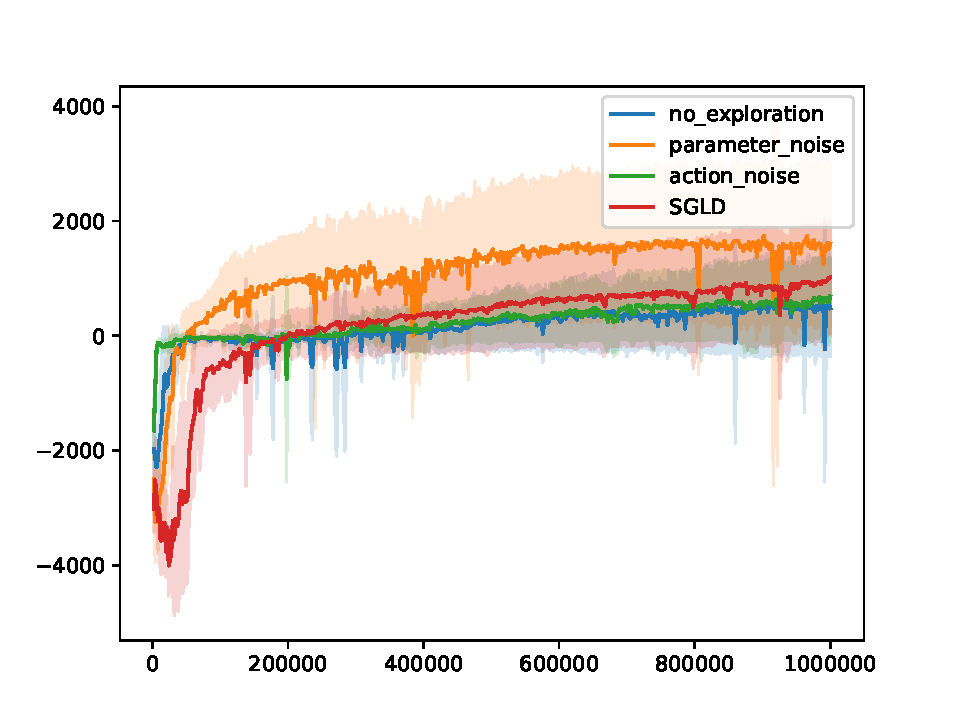
\includegraphics[width=85pt]{figs/HC1.pdf}}
      \subfigure[SHC : $d = 1$]{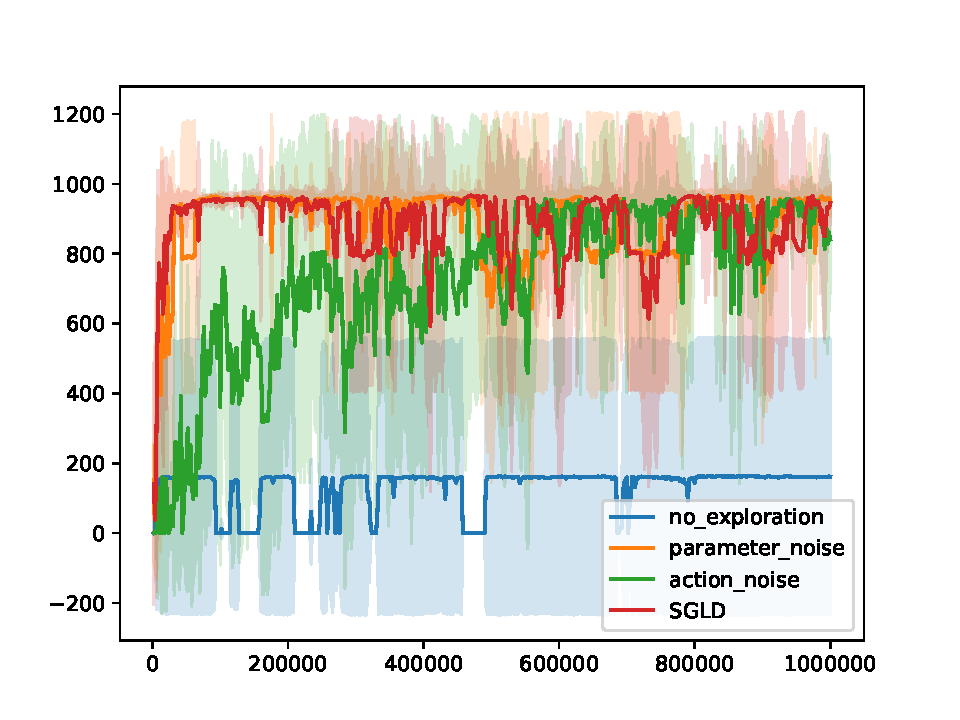
\includegraphics[width=85pt]{figs/SHC1.pdf}}
      \subfigure[SHC : $d = 2.5$]{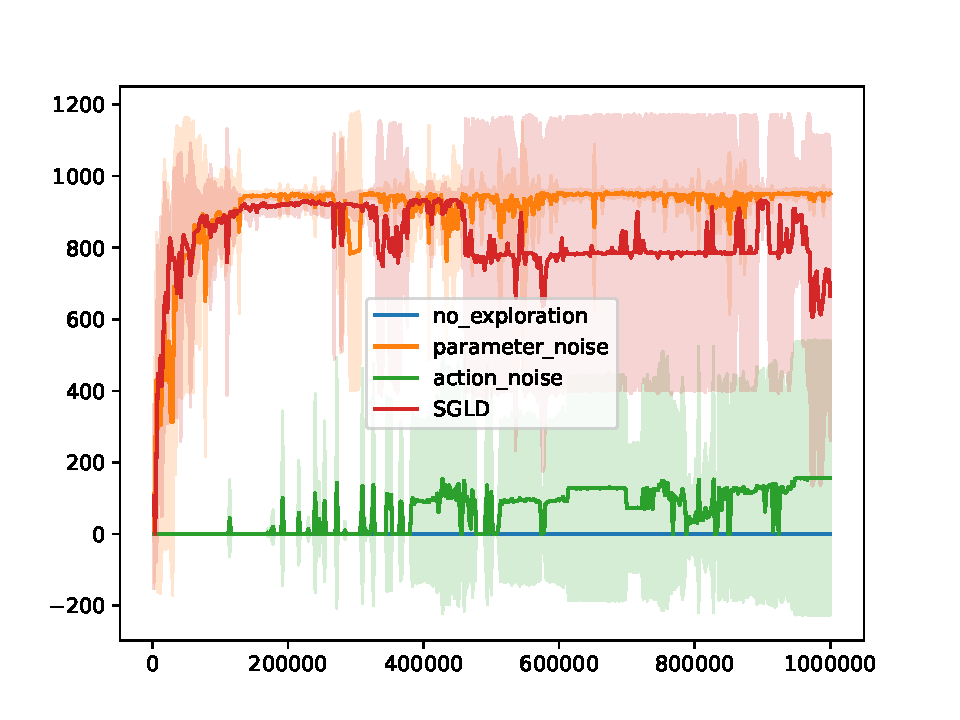
\includegraphics[width=85pt]{figs/SHC2_5.pdf}}
      \subfigure[SHC : $d = 5$]{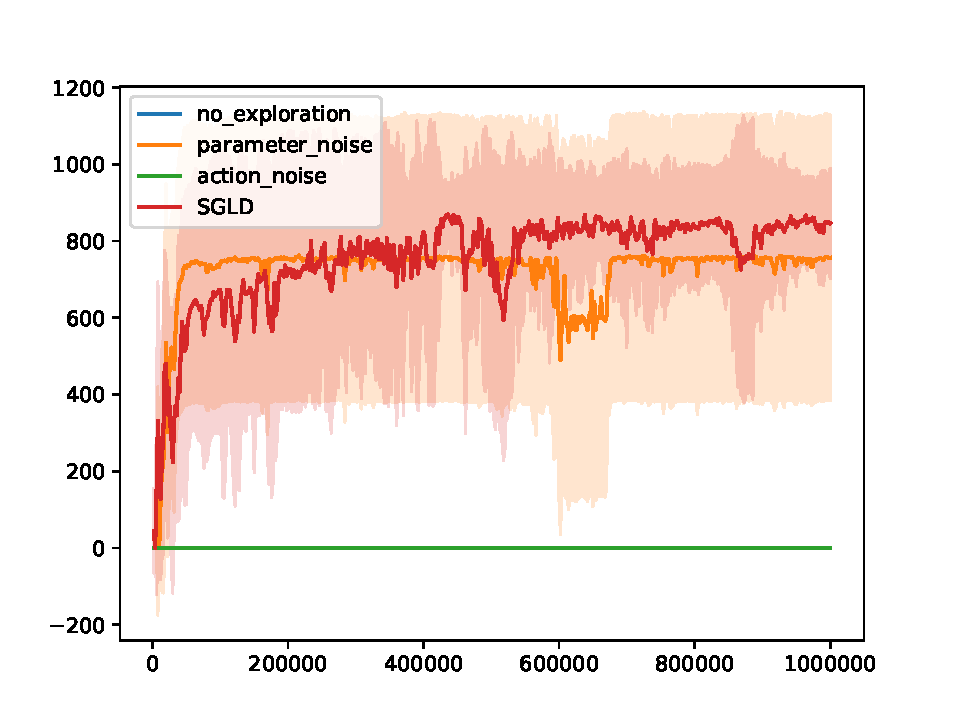
\includegraphics[width=85pt]{figs/SHC.pdf}}
      \subfigure[SHC : $d = 10$]{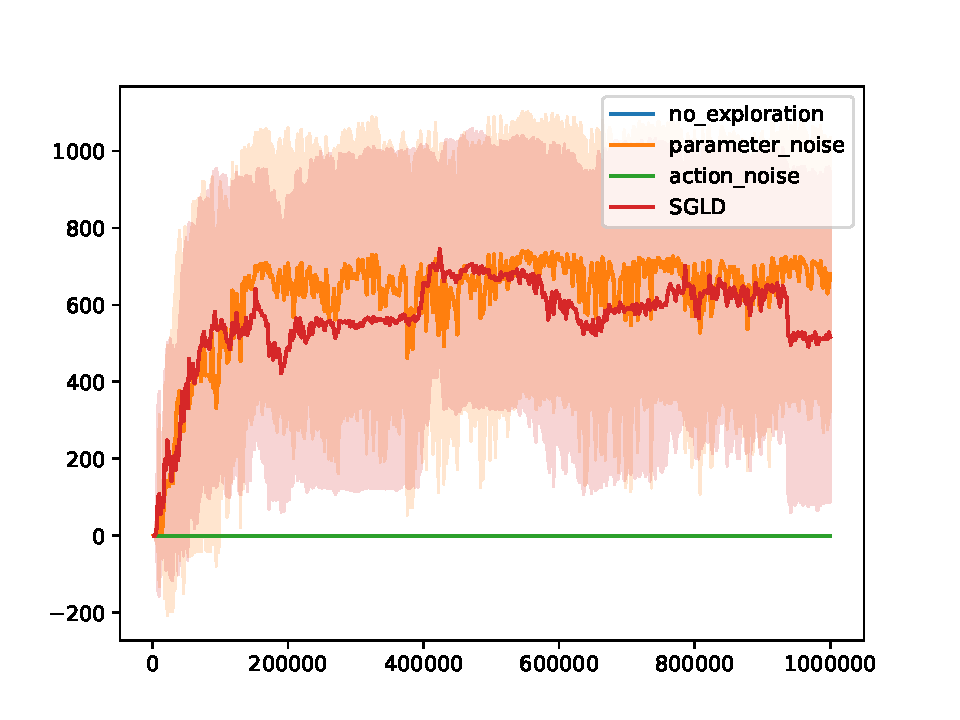
\includegraphics[width=85pt]{figs/SHC10.pdf}}
      \subfigure[SHC : $d = 20$]{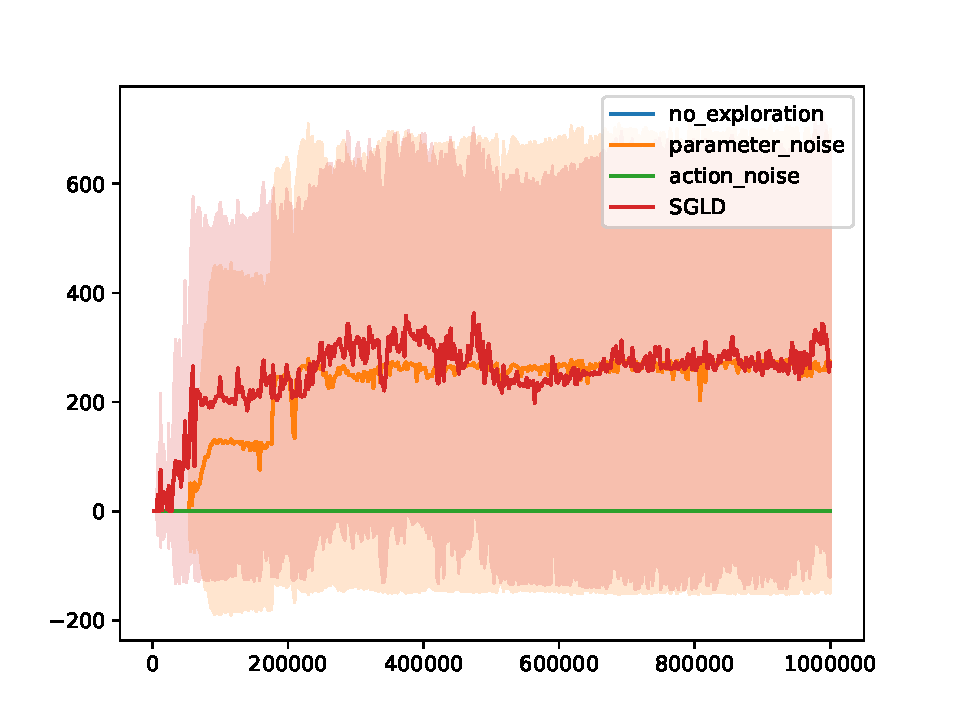
\includegraphics[width=85pt]{figs/SHC20.pdf}}
   \caption{Figures of all experiments. See the appendix for a magnified version.}
   \label{fig:allfigure}   
\end{figure*}

In conclusion: The action noise method succeeded on CMC, but was unable to solve difficult ($d\ge5$) SHC tasks. The parameter noise method succeeded in the SHC task, but failed on the CMC task. The baseline almost failed in all tasks. Our method solved all tasks with a high probability on all settings (minimum 3/6, average 4.9/6). All methods, including the baseline method, can learn to run continuously on the HC with light action penalty. However, as the action penalty increases, the total return attenuation of our method and parameter noise method is slower than the baseline and action noise. The total return of our method and parameter noise method is less reduced, while significant reductions were observed in experiments of baseline and action noise. The figures of all experiments are shown in Figure \ref{fig:allfigure}. The experiment results show that our approach has the best generalization ability on all tasks, and can solve difficult problems and well-defined problems at the same time.

\subsection{Application-Friendly}
It is worth noting that our method does not introduce any hyper-parameters. In the experiments shown above, we use the same settings in all tasks and achieved success in both well-defined tasks and hard tasks, which means lower cost on tuning hyper-parameters.
   
 Our approach also introduces little additional computational cost. We run our method on the HC and compared it to the baseline method. The total running time of the baseline is 5481s, and our method is 5875s. The results show that our method has a close running time compared to the baseline ($1.07\times$), which proves that our method is computational efficient.